\documentclass[10pt,aspectratio=169]{beamer}
\usepackage{tikz}
\usetheme{Boadilla}
\setbeamertemplate{navigation symbols}{}
\title{Geometric uncertainty: experiments and bounds}
\subtitle{Generated interaction study}
\author{Research group}
\date{}
\year=2026\month=11\day=5
\newcommand{\fuzzlayerA}[1]{\textbf{#1}}
\newcommand{\fuzzlayerB}[1]{\fuzzlayerA{#1}}
\newcommand{\fuzzlayerC}[1]{\fuzzlayerB{#1}}
\newcommand{\fuzzterm}[1]{\fuzzlayerC{#1}}
\newcommand{\fuzzpair}[2]{\fuzzterm{#1}: #2}
\newcommand{\fuzzunit}{steps}
\let\fuzzoriginalunit\fuzzunit
\newcommand{\fuzzcoefficient}{2}
\newcommand{\fuzzscale}[2][\fuzzcoefficient]{#1\,#2}
\definecolor{fuzzpaint}{RGB}{255,0,255}
\definecolor{fuzzsecond}{RGB}{18,137,67}
\tikzset{fuzzvertex/.style={draw,rounded corners=1pt,fill=blue!10,inner sep=1pt,minimum width=.35cm,minimum height=.25cm}}
\begin{document}
\section{Geometric uncertainty}
\begin{frame}[t,shrink=5]{Geometric uncertainty}{Composed dependencies}
\fuzzpair{Experiment}{Timing: 12\fuzzunit; estimate $\fuzzscale{x}+\fuzzscale[2]{y}$.}\par
{\renewcommand{\fuzzunit}{samples}\let\fuzzterm\textit\fuzzpair{LocalScope}{Timing: 7\fuzzunit.}\par}
\fuzzpair{RestoredScope}{Timing: 11\fuzzunit.}\par
\begin{columns}[onlytextwidth,b]
\begin{column}{0.46\textwidth}
\begin{itemize}
\item \begin{description}
\item<1->[Stage 1] Before \includegraphics % image argument
[width=20pt,height=10pt,keepaspectratio] % image argument
{fuzz-images/pattern.v2} after.
\item<2->[Stage 2] 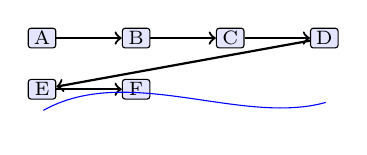
\begin{tikzpicture}[font=\scriptsize]
\begin{scope}[scale=1,rotate=0]


\node[fuzzvertex] (g4n0) at (0.000,0) {A};
\node[fuzzvertex] (g4n1) at (1.195,0) {B};
\node[fuzzvertex] (g4n2) at (2.390,0) {C};
\node[fuzzvertex] (g4n3) at (3.585,0) {D};
\node[fuzzvertex] (g4n4) at (0.000,-0.65) {E};
\node[fuzzvertex] (g4n5) at (1.195,-0.65) {F};
\begin{scope}[xshift=.5pt,yshift=-.5pt]
\draw<1->[->,thick] (g4n0) -- (g4n1);
\draw<1->[->,thick] (g4n1) -- (g4n2);
\draw<1->[->,thick] (g4n2) -- (g4n3);
\draw<1->[->,thick] (g4n3) -- (g4n4);
\draw<1->[->,thick] (g4n4) -- (g4n5);
\draw[blue] (0,-.9) .. controls (1.076,-.3) and (2.510,-1.1) .. (3.585,-.8);
\end{scope}
\end{scope}
\end{tikzpicture}
\end{description}
\item \alt<2->{{\small\color{black}\raggedright
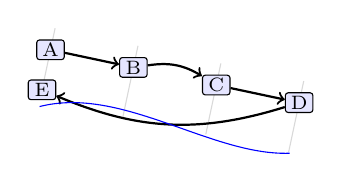
\begin{tikzpicture}[font=\scriptsize]
\begin{scope}[scale=0.8,rotate=-12]

\foreach \x in {0,1,2,3} {\draw[gray!30] (\x*1.345,-.8)--(\x*1.345,.35);}
\node[fuzzvertex] (g7n0) at (0.000,0) {A};
\node[fuzzvertex] (g7n1) at (1.345,0) {B};
\node[fuzzvertex] (g7n2) at (2.690,0) {C};
\node[fuzzvertex] (g7n3) at (4.035,0) {D};
\node[fuzzvertex] (g7n4) at (0.000,-0.65) {E};
\begin{scope}[xshift=.5pt,yshift=-.5pt]
\draw<1->[->,thick] (g7n0) -- (g7n1);
\draw<1->[->,thick] (g7n1) to[bend left=20] (g7n2);
\draw<1->[->,thick] (g7n2) -- (g7n3);
\draw<1->[->,thick] (g7n3) to[bend left=20] (g7n4);
\draw[blue] (0,-.9) .. controls (1.210,-.3) and (2.825,-1.1) .. (4.035,-.8);
\end{scope}
\end{scope}
\end{tikzpicture}\par}}{Alternative estimate $x_0$.}
\item \begin{columns}[onlytextwidth,T]
\begin{column}{0.38\textwidth}
\begin{tikzpicture}\node[draw] {
\includegraphics[page=1,angle=90,width=18pt]{fuzz-images/pages.pdf}};\end{tikzpicture}
\end{column}
\begin{column}{0.58\textwidth}
\begin{tikzpicture}\node[draw] {\includegraphics % image argument
[width=18pt] % image argument
{fuzz-images/pattern.png}};\end{tikzpicture}
\end{column}
\end{columns}
\end{itemize}
\end{column}
\begin{column}{0.50\textwidth}
\begin{columns}[onlytextwidth,b]
\begin{column}{0.62\textwidth}
{\small\color{black}\centering
\begin{enumerate}
\item \begin{description}
\item<1->[Stage 1] Before 
\includegraphics[width=18pt,angle=90]{fuzz-images/pattern.v2} after.
\end{description}
\item \[\begin{pmatrix}a&b\\c&d\end{pmatrix}\begin{pmatrix}x\\y\end{pmatrix}\]
\end{enumerate}\par}
\end{column}
\begin{column}{0.34\textwidth}
{\scriptsize\color{black}\raggedleft
\begin{enumerate}
\item \begin{tabular}{lrr}Method&Cost&Error\\\hline
Cached0&25&6\\
Cached1&17&6\\
\end{tabular}
\item 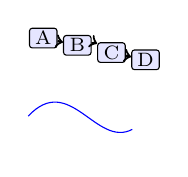
\begin{tikzpicture}[font=\scriptsize]
\begin{scope}[scale=1.1,rotate=-12]


\node[fuzzvertex] (g21n0) at (0.000,0) {A};
\node[fuzzvertex] (g21n1) at (0.402,0) {B};
\node[fuzzvertex] (g21n2) at (0.805,0) {C};
\node[fuzzvertex] (g21n3) at (1.207,0) {D};
\begin{scope}[xshift=.5pt,yshift=-.5pt]
\draw<2->[->,thick] (g21n0) -- (g21n1);
\draw<2->[->,thick] (g21n1) to[bend left=20] (g21n2);
\draw<2->[->,thick] (g21n2) -- (g21n3);
\draw[blue] (0,-.9) .. controls (0.362,-.3) and (0.845,-1.1) .. (1.207,-.8);
\end{scope}
\end{scope}
\end{tikzpicture}
\item Before 
\includegraphics[trim=2 1 3 2,viewport=1 1 20 14,clip=false]{fuzz-images/pattern.png} after.
\end{enumerate}\par}
\end{column}
\end{columns}
\end{column}
\end{columns}
\par 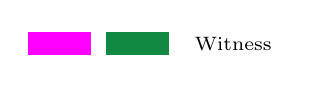
\begin{tikzpicture}[font=\scriptsize]
\fill<2-3>[fuzzpaint] (0,0) rectangle (.8,.3);
\fill<3->[fuzzsecond] (1,0) rectangle (1.8,.3);
\node[anchor=west] at (2,0.15) {Witness};
\end{tikzpicture}
\only<4>{}
\end{frame}
\renewcommand{\fuzzunit}{Hz}
\renewcommand{\fuzzcoefficient}{2}
\renewcommand{\fuzzterm}[1]{{\textrm{#1}}}
\section{Geometric uncertainty}
\begin{frame}[t]{Iterative refinement}
\fuzzpair{MacroStageB}{Timing: 12\fuzzunit, retained: 9\fuzzoriginalunit.}\par
{\renewcommand{\fuzzunit}{local}\fuzzpair{FrameLocal}{Timing: 5\fuzzunit.}\par}
\fuzzpair{FrameRestored}{Timing: 8\fuzzunit; estimate $\fuzzscale{x}$.}\par
\begin{columns}[T]\begin{column}{.46\textwidth}We compare the proposed solution with a reference computed from the complete input.\end{column}\begin{column}{.46\textwidth}\begin{itemize}\item Input state\item Updated state\end{itemize}\end{column}\end{columns}
\end{frame}
\renewcommand{\fuzzunit}{us}
\renewcommand{\fuzzcoefficient}{3}
\renewcommand{\fuzzterm}[1]{{\textrm{#1}}}
\section{Geometric uncertainty}
\begin{frame}[t]{Constraint propagation}
\fuzzpair{MacroStageC}{Timing: 12\fuzzunit, retained: 9\fuzzoriginalunit.}\par
{\renewcommand{\fuzzunit}{local}\fuzzpair{FrameLocal}{Timing: 5\fuzzunit.}\par}
\fuzzpair{FrameRestored}{Timing: 8\fuzzunit; estimate $\fuzzscale{x}$.}\par
\begin{block}{Follow-up}\fuzzterm{A revised value} depends on the preceding frame.\end{block}
\[r_{k+1}=r_k-\alpha d_k\]
\end{frame}
\end{document}
